% -*- Mode:TeX -*-

%% The documentclass options along with the pagestyle can be used to generate
%% a technical report, a draft copy, or a regular thesis.  You may need to
%% re-specify the pagestyle after you \include  cover.tex.  For more
%% information, see the first few lines of mitthesis.cls. 

%\documentclass[12pt,vi,twoside]{mitthesis}
%%
%%  If you want your thesis copyright to you instead of MIT, use the
%%  ``vi'' option, as above.
%%
%\documentclass[12pt,twoside,leftblank]{mitthesis}
%%
%% If you want blank pages before new chapters to be labelled ``This
%% Page Intentionally Left Blank'', use the ``leftblank'' option, as
%% above. 

%\documentclass[12pt,twoside]{mitthesis}
\documentclass[12pt]{mitthesis}
%\documentclass[12pt,twoside,leftblank]{mitthesis}
% NOTE! For printing two-sided, include twoside in document class!
\usepackage{lgrind}
%\usepackage{mathpazo}

%\usepackage[T1]{fontenc}
%\usepackage[sc]{mathpazo}
%\linespread{1.05} 
% Euler for math | Palatino for rm | Helvetica for ss | Courier for tt
\renewcommand{\rmdefault}{ppl} % rm
%\linespread{1.05}        % Palatino needs more leading
\usepackage[scaled]{helvet} % ss
\usepackage{courier} % tt
\usepackage{euler} % math
%\usepackage{eulervm} % a better implementation of the euler package (not in gwTeX)
\normalfont
\usepackage[T1]{fontenc}
\usepackage{subfig}
\usepackage{graphicx}
\usepackage{color}
\usepackage{listings}
\usepackage{verbatim}
\usepackage{longtable}
\usepackage{hyphenat}
\usepackage[section]{placeins}
\usepackage{hyperref}
\usepackage{multicol}
\usepackage{multirow}
\usepackage{pdfpages}
\usepackage{epstopdf}
%\setcounter{topnumber}{2}
%\setcounter{bottomnumber}{2}
%\setcounter{totalnumber}{4}
%\renewcommand{\topfraction}{0.85}
%\renewcommand{\bottomfraction}{0.85}
%\renewcommand{\textfraction}{0.15}
%\renewcommand{\floatpagefraction}{0.7}

\newcommand{\opref}[1]{\nohyphens{#1}}
\newcommand{\fieldref}[1]{\nohyphens{\tt #1}}
\newcommand{\opfield}[2]{\fieldref{#1} & \opref{#2} \\ \hline}

\newcommand{\inst}[1]{{\em #1}}
\newcommand{\bnfmeta}[1]{{\Large #1}}
\newcommand{\bnfterm}[1]{{\sf\bfseries #1}}

\newcommand{\tablehead}[1]{{\bf #1}}
\hypersetup{
    colorlinks=false,
    pdfborder={0 0 0},
}

\sloppy

\lstset{language=Python}
\DeclareGraphicsExtensions{.pdf}
\graphicspath{{./performance/pdf/}{./figures/pdf-perm/}{./figures/dot/}}
\pagestyle{plain}

\newenvironment{pseudo}
               {\begin{figure}[ht]
                   \rule{\textwidth}{1pt}
                   }               
               {\rule{\textwidth}{1pt} 
               \end{figure}}
\newenvironment{wspec}[0]
               {\begin{center}\begin{minipage}{.9\textwidth}
               }{\end{minipage}
                 \end{center}
               }

\def\sectionautorefname{Section}
\def\chapterautorefname{Chapter}
\def\subsectionautorefname{Section}
\def\subsubsectionautorefname{Section}

\lstset{
  basicstyle=\ttfamily \small,
  showstringspaces=false,
  linewidth=0.9\textwidth,
  breaklines=true,
  breakatwhitespace=true,
}

\lstdefinelanguage{ANTLR}{
  basicstyle=\ttfamily \footnotesize,
  keywordstyle=\bf,
  morekeywords={},
  stringstyle=\bf,
  morestring=[b]",
  morestring=
}

\lstdefinelanguage{WSL}{
  basicstyle=\ttfamily\small,
  keywordstyle=\bf\rmfamily,
  keywordstyle=[2]\bf\rmfamily,
  morekeywords={[2]ON, ADD, REMOVE},
  morekeywords={OR, AND, IN, CONTAINS},
%  frameround=tttt,
%  frame=tlrb,
%  linewidth=0.9\textwidth,
%  xleftmargin=.5em,
%  breaklines=true,
%  breakatwhitespace=true
}

\begin{document}

% -*-latex-*-
% 
% For questions, comments, concerns or complaints:
% thesis@mit.edu
% 
%
% $Log: cover.tex,v $
% Revision 1.8  2008/05/13 15:02:15  jdreed
% Degree month is June, not May.  Added note about prevdegrees.
% Arthur Smith's title updated
%
% Revision 1.7  2001/02/08 18:53:16  boojum
% changed some \newpages to \cleardoublepages
%
% Revision 1.6  1999/10/21 14:49:31  boojum
% changed comment referring to documentstyle
%
% Revision 1.5  1999/10/21 14:39:04  boojum
% *** empty log message ***
%
% Revision 1.4  1997/04/18  17:54:10  othomas
% added page numbers on abstract and cover, and made 1 abstract
% page the default rather than 2.  (anne hunter tells me this
% is the new institute standard.)
%
% Revision 1.4  1997/04/18  17:54:10  othomas
% added page numbers on abstract and cover, and made 1 abstract
% page the default rather than 2.  (anne hunter tells me this
% is the new institute standard.)
%
% Revision 1.3  93/05/17  17:06:29  starflt
% Added acknowledgements section (suggested by tompalka)
% 
% Revision 1.2  92/04/22  13:13:13  epeisach
% Fixes for 1991 course 6 requirements
% Phrase "and to grant others the right to do so" has been added to 
% permission clause
% Second copy of abstract is not counted as separate pages so numbering works
% out
% 
% Revision 1.1  92/04/22  13:08:20  epeisach

% NOTE:
% These templates make an effort to conform to the MIT Thesis specifications,
% however the specifications can change.  We recommend that you verify the
% layout of your title page with your thesis advisor and/or the MIT 
% Libraries before printing your final copy.
\title{Summarizing Audit Trails in the Aeouls Security Platform}

\author{Wissam Jarjoui}
% If you wish to list your previous degrees on the cover page, use the 
% previous degrees command:
%       \prevdegrees{A.A., Harvard University (1985)}
% You can use the \\ command to list multiple previous degrees
%       \prevdegrees{B.S., University of California (1978) \\
%                    S.M., Massachusetts Institute of Technology (1981)}
\prevdegrees{S.B., C.S M.I.T., 2011}
\department{Department of Electrical Engineering and Computer Science}

% If the thesis is for two degrees simultaneously, list them both
% separated by \and like this:
% \degree{Doctor of Philosophy \and Master of Science}
\degree{Master of Engineering in Electrical Engineering and Computer Science}

% As of the 2007-08 academic year, valid degree months are September, 
% February, or June.  The default is June.
\degreemonth{September}
\degreeyear{2012}
\thesisdate{August 15, 2012}

%% By default, the thesis will be copyrighted to MIT.  If you need to copyright
%% the thesis to yourself, just specify the `vi' documentclass option.  If for
%% some reason you want to exactly specify the copyright notice text, you can
%% use the \copyrightnoticetext command.  
%\copyrightnoticetext{\copyright IBM, 1990.  Do not open till Xmas.}

% If there is more than one supervisor, use the \supervisor command
% once for each.
\supervisor{Barbara H. Liskov}{Institute Professor}

% This is the department committee chairman, not the thesis committee
% chairman.  You should replace this with your Department's Committee
% Chairman.
\chairman{Christopher J. Terman}{Chairman, Masters of Engineering Thesis Committee}

% Make the titlepage based on the above information.  If you need
% something special and can't use the standard form, you can specify
% the exact text of the titlepage yourself.  Put it in a titlepage
% environment and leave blank lines where you want vertical space.
% The spaces will be adjusted to fill the entire page.  The dotted
% lines for the signatures are made with the \signature command.
\maketitle

% The abstractpage environment sets up everything on the page except
% the text itself.  The title and other header material are put at the
% top of the page, and the supervisors are listed at the bottom.  A
% new page is begun both before and after.  Of course, an abstract may
% be more than one page itself.  If you need more control over the
% format of the page, you can use the abstract environment, which puts
% the word "Abstract" at the beginning and single spaces its text.

%% You can either \input (*not* \include) your abstract file, or you can put
%% the text of the abstract directly between the \begin{abstractpage} and
%% \end{abstractpage} commands.

% First copy: start a new page, and save the page number.
\cleardoublepage
% Uncomment the next line if you do NOT want a page number on your
% abstract and acknowledgments pages.
% \pagestyle{empty}
\setcounter{savepage}{\thepage}
\begin{abstractpage}
% $Log: abstract.tex,v $
% Revision 1.1  93/05/14  14:56:25  starflt
% Initial revision
% 
% Revision 1.1  90/05/04  10:41:01  lwvanels
% Initial revision
% 
%
%% The text of your abstract and nothing else (other than comments) goes here.
%% It will be single-spaced and the rest of the text that is supposed to go on
%% the abstract page will be generated by the abstractpage environment.  This
%% file should be \input (not \include 'd) from cover.tex.
Aeolus is a programming platform that supports the development of secure applications that preserve the confidentiality of information entrusted to them. An important part of the Aeolus platform is an auditing subsystem that maintains a log in which it stores information about every security related event that occurs while applications run. The log allows later analysis to determine whether the security policies of the application have been followed.

For an Aeolus user, analyzing an Aeolus event log can prove to be a daunting task, especially when this log grows to include millions of records. Similarly, storing such an event log can be very costly. The system I present in this thesis provides an interface that allows the creation of user-defined summaries of the Aeolus audit trails, as well as marking of events in the log for future archiving or deletion. Our system makes it easier to analyze the Aeolus event log and less costly to store events of interest. This is done through the use of a \emph{QuerySystem} and \emph{SummaryObjects}.
I present the system in the context of a sample application based on the financial management service \emph{www.mint.com}. The system is an extension to the Aeolus library; it is implemented in Java code and uses PostgreSQL 9.0 as its primary database.





\end{abstractpage}

% Additional copy: start a new page, and reset the page number.  This way,
% the second copy of the abstract is not counted as separate pages.
% Uncomment the next 6 lines if you need two copies of the abstract
% page.
% \setcounter{page}{\thesavepage}
% \begin{abstractpage}
% % $Log: abstract.tex,v $
% Revision 1.1  93/05/14  14:56:25  starflt
% Initial revision
% 
% Revision 1.1  90/05/04  10:41:01  lwvanels
% Initial revision
% 
%
%% The text of your abstract and nothing else (other than comments) goes here.
%% It will be single-spaced and the rest of the text that is supposed to go on
%% the abstract page will be generated by the abstractpage environment.  This
%% file should be \input (not \include 'd) from cover.tex.
Aeolus is a programming platform that supports the development of secure applications that preserve the confidentiality of information entrusted to them. An important part of the Aeolus platform is an auditing subsystem that maintains a log in which it stores information about every security related event that occurs while applications run. The log allows later analysis to determine whether the security policies of the application have been followed.

For an Aeolus user, analyzing an Aeolus event log can prove to be a daunting task, especially when this log grows to include millions of records. Similarly, storing such an event log can be very costly. The system I present in this thesis provides an interface that allows the creation of user-defined summaries of the Aeolus audit trails, as well as marking of events in the log for future archiving or deletion. Our system makes it easier to analyze the Aeolus event log and less costly to store events of interest. This is done through the use of a \emph{QuerySystem} and \emph{SummaryObjects}.
I present the system in the context of a sample application based on the financial management service \emph{www.mint.com}. The system is an extension to the Aeolus library; it is implemented in Java code and uses PostgreSQL 9.0 as its primary database.





% \end{abstractpage}

\cleardoublepage

\section*{Acknowledgments}

First and foremost, I would like to thank my advisor, Prof. Barbara Liskov, for the mentorship she gave me in my two years here at PMG. Her guidance helped me navigateand learn a lot about systems security, and went beyond just this project. I am truely grateful for the understanding, patience and investment she put in while helping me see this project through; I hope that one day I would be able to reflect those traits as a leader.

A big thank you to my colleague, David Schultz, for his tremendous help in this project and my personal learning; from suggesting and brainstorming ideas to improve my project, to explaining technical concepts, and being a strong source of knowledge and inspiration and a good role model in general. David, it has been a pleasure working with you.

I would also like to thank James Cowling, Dan Ports and Barzan Mozafari and everyone in 32-G908 for all the fun conversations and advice they provided. I am very fortunate to have had the chance to hear and learn from their experiences, and be inspired by them.

As this thesis culminates five years for me at MIT, firstly I would like to take this chance to also thank my friends for being their for me, and for offering me help even when I didn't ask. Their presence was a home away from home, and their support guided me in times of uncertainty. Secondly, I would like to thank my family; I would not be where I am today if it were not for them. I thank them for their support and encouragement, for worrying about the things I wouldn't, and for setting the bar high. In one way or another, I will always have something to learn from them.

Finally, I would like to thank MIT for all what it has given me -- Anne Hunter, my advisors, my professors and my TAs. I thank Stata and the Infinite for being monuments of my experience here at MIT, and I thank the Charles River, for being the source of calmness in a very busy time. They will all be missed.


%%%%%%%%%%%%%%%%%%%%%%%%%%%%%%%%%%%%%%%%%%%%%%%%%%%%%%%%%%%%%%%%%%%%%%
% -*-latex-*-

% Some departments (e.g. 5) require an additional signature page.  See
% signature.tex for more information and uncomment the following line if
% applicable.
% % -*- Mode:TeX -*-
%
% Some departments (e.g. Chemistry) require an additional cover page
% with signatures of the thesis committee.  Please check with your
% thesis advisor or other appropriate person to determine if such a 
% page is required for your thesis.  
%
% If you choose not to use the "titlepage" environment, a \newpage
% commands, and several \vspace{\fill} commands may be necessary to
% achieve the required spacing.  The \signature command is defined in
% the "mitthesis" class
%
% The following sample appears courtesy of Ben Kaduk <kaduk@mit.edu> and
% was used in his June 2012 doctoral thesis in Chemistry. 

\begin{titlepage}
\begin{large}
This doctoral thesis has been examined by a Committee of the Department
of Chemistry as follows:

\signature{Professor Jianshu Cao}{Chairman, Thesis Committee \\
   Professor of Chemistry}

\signature{Professor Troy Van Voorhis}{Thesis Supervisor \\
   Associate Professor of Chemistry}

\signature{Professor Robert W. Field}{Member, Thesis Committee \\
   Haslam and Dewey Professor of Chemistry}
\end{large}
\end{titlepage}


\pagestyle{plain}
  % -*- Mode:TeX -*-
%% This file simply contains the commands that actually generate the table of
%% contents and lists of figures and tables.  You can omit any or all of
%% these files by simply taking out the appropriate command.  For more
%% information on these files, see appendix C.3.3 of the LaTeX manual. 
\tableofcontents
%\newpage
%\listoffigures
%\newpage
%\listoftables


%% This is an example first chapter.  You should put chapter/appendix that you
%% write into a separate file, and add a line \include{yourfilename} to
%% main.tex, where `yourfilename.tex' is the name of the chapter/appendix file.
%% You can process specific files by typing their names in at the 
%% \files=
%% prompt when you run the file main.tex through LaTeX.
\chapter{Introduction}

Security of confidential online information, such as medical records and financial data, is a very important problem. Recent research has focused on Cecentralized Information Flow Control (DIFC) as the most promising approach to enable application developers to secure information. DIFC is based on the principle that the system tracks information as it flows through the system, and only allows release if the releaser has sufficient authority. Additionally DIFC provides this ability in a fine-grained way, so that security policies can be tailored to the needs of individual users and organizations.

This thesis extends the security support provided by the Aeolus platform. Aeolus is a platform that combines DIFC and an intuitive security model framework to make it more convenient for developers to build secure applications on a distributed system. Additionally Aeolus provides automatic auditing of every security related event that occurs while an application runs; also it provides a way for applications to log additional events that are meaningful at the application level. The audit trail is an important component of security to allow discovery of errors that cause security policies to be subverted; the audit trail can also be used to discover attacks.

Aeolus allows application developers to track information flow by logging information about the processes running in the application, as well as the operations they carry out. This provides developers with a complete history of the application's activity and information flow through the system since startup. This log is called the \emph{event log}.

The event log is a causal graph: each ``event'' that took place in the system has predecessors, and hence developers can construct an event graph and analyze it to identify causes of information leakage. However, logging all process operations for a distributed system can produce a very large event log very quickly. Analyzing and storing such an event log can prove to be both daunting and costly for an application developer, and calls for providing an Aeolus application developer with easier access to information about events of interest.

In this thesis I present a system built on top of the Aeolus security platform that allows users to create \emph{summaries} of the event log. These summaries are application-specific, and left up to the developer to define. What our system provides is a simple framework for the developer to reason about creation, storage and modification of these summaries, as well as archiving of the original event log.

The next two sections describe the motivation and scope of this system with the help of some real-life examples.

Chapter 2 presents an overview of the Aeolsu security system. Chapter 3 presents a sample Aeolus application based on Mint.com.

Chapter 4 describes the summarization and archiving models and interfaces.

Chapter 5 describes the implementation details of the system.

Chapter 6 evaluates the ease of use of the system as well as overall system performance.

Chapter 7 discusses related work in streaming databases.

Chapter 8 presents some topics for future work and reviews the contributions of this thesis.

Appendix A details the summarization and archiving interface and presents some examples.


\section{Motivation for summarization and archival}

The Aeolus platform logs all events that take place in the system. Despite the fact that these events can tell you everything that happened in the system, they do not carry any semantic meaning. Allowing application developers to define a semantic meaning for events, or groups of events, helps in analyzing the history of the system.

Take for example a bank's web administrator who is interested in auditing outbound transfers from customers' web accounts. A straighfoward way to do this is to plot the number of outbound transfers carried through a user's account for each week in the last year. Any spikes in the rate outboud transactions per week could mean that a user's account has been compromised by an attacker. A sample graph is presented in figure x.x.

Producing such information is absolutely possible through the current auditing mechanisms available in Aeolus. However, in order to accomplish such a task, the adminsitrator will not only have to scan all events in the system, but will also, most likely, have to do this frequently to keep his audit records up to date.

Summarization solves these problems by allowing developers to focus on scanning and analyzing only events of interest. Creating and storing \emph{event summaries} also paves the way for archival: now the web administrator in the example above can choose to archive events that more than a year old - if they are \emph{sufficiently summarized} (perhaps footnote a definition of event summaries + sufficiently summarized here).

\section{Scope}

As security platform developers, tackling the problem of summarization and archival raises a number of questions: what usage scenarios are we trying to satisfy? How do we generalize our model to satisfy those scenarios? What guarantees do we provide to our developers? And how do we maintain those guarantees?

I will start by stating that our system, similar to the Aeolus security platform itself, assumes an application developer to be active and aware of the workings of Aeolus as a whole. We do not intend for our system to impose any restrictions on the developer, and hence the developer would have to be careful with the power granted to them through the our system.

Those are the basic assumptions we made while building the system, and most design decisions stem from them. While reading the following chapters, the reader should expect to gain a better understanding of the definitions of the questions posed above, the design problems they pose, and how we answer them.

\chapter{Aeolus System Overview}
\label{aeolus}

This chapter presents an overview of the Aeolus security platform, on which our summarization system is based, and highlights relevant details such as log collection. More complete descriptions of the Aeolus security platform and its log collection and analysis can be found in Cheng \cite{cheng}, Popic \cite{popic} and Blankstein \cite{blanks}.

\section{System Architecture}

\begin{figure}[ht]
\centering
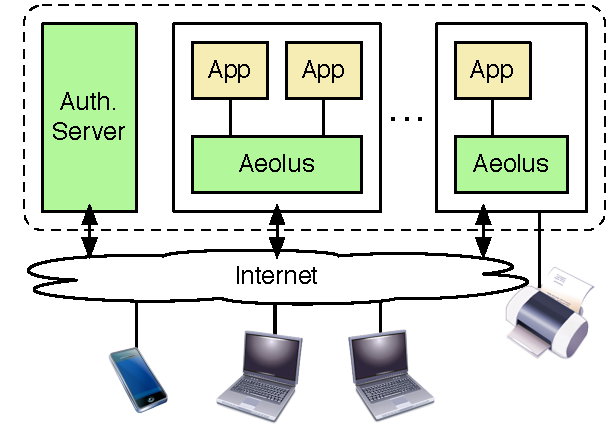
\includegraphics[bb= 0 0 292 204, width=.5\textwidth]{figures/sysarch}
\caption*{Aeolus System Architecture}
\caption[Aeolus System Architecture]{High level overview of Aeolus system architecture.}
\label{fig:aeolus-sysarch}
\end{figure}

The Aeolus architecture is shown in figure \ref{fig:aeolus-sysarch}. The system consists of many nodes, each of which is trusted to enforce Aeolus's information flow rules.

Aeolus tracks information flow within each system node and between system nodes. Nodes in the system communicate via RPC messages, those messages are encrypted to protect their secrecy and integrity. Nodes outside the system are considered to be untrusted: information can flow outside of the system only if it is uncontaminated, and information arriving from the outside is marked as having no integrity.


Threads in Aeolus run on behalf of \emph{principals}. The ability of a thread to carry out \emph{privileged operations} is determined by the \emph{authority} of the principal it runs on behalf of. Aeolus tracks the authority of principals in the \emph{authority state} stored at the authority server (AS). Principals, privileged operations and authority are described in sections \ref{principals}, \ref{difc:rules} and \ref{auth}, respectively.

\section{Information Flow Model}

This section describes the basic concepts and rules of the Aeolus security model.

\subsection{Prinicpals, Tags and Labels}\label{principals}

Aeolus employs an intuitive security model to implement information flow control. The model revolves around three key concepts: \emph{principals}, \emph{tags} and \emph{labels} \cite{aeolus}. Principals represent entities in the system that create, modify and share information. Tags represent security categories of information. A principal authoritative for a certain tag can modify or share information categorized by that tag. Labels are sets of tags and are used to determine whether information can flow from a source to a receiver based on the information flow rules described in the following section.

\subsection{Information Flow Rules}\label{difc:rules}

Aeolus allows information to flow from a source \emph{S} to a destination \emph{D} only if the following rules are satisfied:

\begin{eqnarray*}
  SECRECY_{S} &\subseteq& SECRECY_{D} \\
  INTEGRITY_{S} &\supseteq& INTEGRITY_{D}
\end{eqnarray*}

Threads in an Aeolus node run with security and integrity labels associated with them; objects such as files also have such labels. In Aeolus, a thread cannot modify labels of files or shared memory objects; however, the labels of threads can change, and hence a thread would have to modify it's own labels in order to read or write data. 

Certain label manipulations, called \emph{privileged manipulations} are unsafe because they remove constraints on information flow:

\begin{enumerate}
  \item \emph{Declassfication} Remove a tag from a secrecy label.
  \item \emph{Endorsement} Add a tag to an integrity label.
\end{enumerate}

\noindent
A thread is allowed to carry out privileged label manipulations if it is running on behalf of a principal that has authority for the tags affected by these manipulations.

\subsection{Authority}\label{auth}

Authority determines whether a thread can perform privileged label manipulations. Authority starts with tag creation: when a thread creates a tag, its principal has authority for that tag.

Subsequently, the Aeolus authority state can be modified through \emph{grant}, \emph{act-for} or \emph{revoke} operations. Grant operations allow a principal to delegate authority for a particular tag to another principal. \emph{Act-for} operations allow a principal to delegate all of its authority to another principal. Revoke operations remove \emph{act-for} and \emph{grant} links between principals. To avoid covert channels, Aeolus only permits threads running with null secrecy labels to modify the authority state.

\subsection{Compound Tags}

Applications frequently have sets of tags that are closely related. In order to simplify the authority structure of the application, Aeolus allows for tags to be grouped upon creation using \emph{compound tags}. For example, in a medical clinic, patient data tags are \emph{subtags} of an \emph{ALL-PATIENT-DATA} tag, a \emph{supertag}.

A principal authoritative for a supertag is also authoritative for all of its subtags. Similarly, having a supertag in a thread's secrecy label is equivalent to having all subtags in its secrecy label. This reduces label size substantially, and makes label manipulations involving paricular groups of tags less expensive.


See figure \ref{fig:mint-auth-state-model} on page \pageref{fig:mint-auth-state-model} for an example of an authority state model, detailing \emph{act-for}, \emph{grant} and \emph{subtag} relationships in the financial services application described in chapter \ref{mint}.

\section{Programming Model}

This section explains the programming abstraction Aeolus provides, and how they support DIFC.

\subsection{Threads and Vitual Nodes}

Virtual nodes (VNs), shown as applications in figure \ref{fig:aeolus-sysarch}, communicate via RPC and have many threads inside them. A VN is given a principal when it is created and all threads run with this principal or some prinicipal it acts for. An RPC is run in its own threads with the VN prinicipal but the labels of the caller; on the return the labels are sent back to the caller where they are merged with those of the caller: a merge is a union of the secrecy labels and an intersection of the integrity labels. Then the caller continues with its own principal.

\subsection{Shared State Objects and Boxes}\label{aeolus:shared-mem}

Within a virtual node, threads can share state via special Aeolus shared objects. Aeolus gives threads access to a \emph{root} shared memory object, with null labels.

Aeolus shared obects have immutable labels, and Aeolus ensures that the rules in \ref{difc:rules} are respected. User's can create their own shared objects; Aeolus ensures that label manipulations do not take place inside the object's methods.

\subsection{Authority Closures and Reduced Authority Calls}
\label{aeolus:auth-calls}

Aeolus provides developers with \emph{authority closures}. An authority closure is an object bound to a principal at the moment of creation. Threads can later call the closure's methods, which run with the closure's principal. Authority closures allow threads to process confidential information without being exposed to the information itself.

Aeolus also provides a mechanism for threads to reduce their authority, called \emph{reduced authority calls}. To make a reduced authority call, a thread specifies a function and a principal to run it with. The calling thread's principal must act for the principal of the reduced authority call.

With those two mechanisms in place, Aeolus makes it possible to ensure that each part of the application runs with only the authority it needs. Aeolus also provides a principal that is not authoritative for any tags, \emph{P$_{PUBLIC}$}, for developers to use when they need to ensure that a part of a program cannot leak any information.

\subsection{Files}

Aeolus provides a network file system that enforces DIFC. Similarly to shared memory objects, files have immutable labels and the rules in \ref{difc:rules} apply for information flow in and out of them.

Files are yet another way (RPCs, shared memoery objects) through which Aeolus allows threads to communicate. A complete description of the Aeolus file system API is presented in McKee \cite{mckee}.

\subsection{Log Collection}

\begin{figure}[h]
\centering
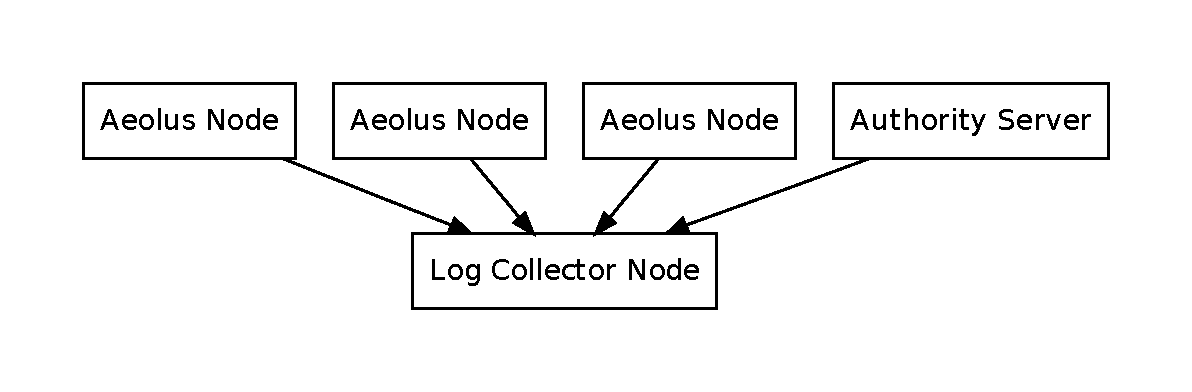
\includegraphics[height=7em]{figures/event-logging-overview}
\caption*{Log Collection}
\caption[Aeolus Log Collection]{Flow of logs to the log collection system.}
\label{fig:log-flow}
\end{figure}

Aeolus provides automatic auditing of every security related event that occurs while an application runs; also it provides a way for applications to log additional events that are meaningful at the application level.

Aeolus distributes log collection across all nodes in the system. Aeolus sends events that occur locally to the log collector as shown in figure \ref{fig:log-flow}. The log collector stores the events for later processing and analysis, as explained in \cite{blanks}.

Aeolus provides application-level logging to allow developers to log their own events using the following interface:

\begin{lstlisting}[language=Java, label=app-logging]
AeolusLib.createEvent(String app_op, List<String> args)
\end{lstlisting}

\noindent
This creates a new record in the Aeolus event log. The \emph{app\_op} and \emph{args} argument are stored as attributes for that record, allowing the developer to query the event log based on the arguments they provided. The \emph{app\_op} parameter is used to to identify the application operation name, and the \emph{args} paramter allows the developer to specify any additional information to store for the event.

\subsubsection{Aeolus Event Attributes}
\label{sec:aeolus-event-attributes}
Aeolus stores different attributes for different events that take place in the system. Blankstein \cite{blanks} provides a complete description of those attributes; here we will highlight the ones more relevant to the use of summarization:

\begin{description}
  \item[\emph{event\_counter}] \ \\
    The event counter uniquely identifies an event, and provides an
    ordering for the occurence of the event, i.e. events with a higher 
    eventcounter took place after events with a lower eventcounter.
  \item[\emph{timestamp}] \ \\
    This is the real time at which the event happened.
  \item[\emph{secrecy}] \ \\
    This is the secrecy label of the thread which caused the event, 
    just before the event took place.
  \item[\emph{integrity}] \ \\
    This is the integrity label of the thread which caused the event, 
    just before the event took place.
  \item[\emph{op\_name}] \ \\
    This field specifies the type of the event, 
    e.g. a \emph{DECLASSIFY} event, 
    or a \emph{SENDRPC} event. Those types are 
    detailed in \cite{blanks}.
    Application-level events created with the above events
    all have the \emph{APPLICATION\_LVL} operation name.
  \item[\emph{app\_op}] \ \\
    This field holds the name of the 
    application-specific operation and is 
    provided by the developer as described above.
  \item[\emph{app\_args}] \ \\
    This field holds the arguments specified for an application-level 
    event (the second argument in the interface shown above).
  \item[\emph{running\_principal}] \ \\
    This field holds the principal of the thread that caused the event.
\end{description}

It is important to note that the \emph{secrecy} and \emph{integrity} attributes are particularly import to prevent information leakage in the system: a thread can only read those event records if the DIFC rules in \ref{difc:rules} are satisfied.

% The audit trail is an important component of security to allow discovery of errors that cause security policies to be subverted; the audit trail can also be used to discover attacks.

%\subsection{Priviledged Operations}

%Certain label modifications are \emph{priviledged operations}: removing a tag from the secrecy label and adding a tag to the integrity label. If a process is running on behalf of a principal authoritative for a certain tag, then that process can carry priviledged operations on that tag.

%\subsection{Information Flow in and out of the System}

%Aeolus process can only write outside the system boundaries if it has empty labels. This restriction combined with the information flow rules in \ref{difc:rules} ensures that a process can only expose information if it is running on behalf of a principal authoritative for tags categorizing that information.

%Aeolus virtual nodes can use RPC to communicate with one another, and Aeolus threads can communicate using shared state mechanisms. Aeolus enforces that both of these communication mechanisms abide by the rules in \ref{difc:rules}.

%\section{Log Collection}

%Aeolus nodes are responsible for logging any events that occur locally, and sending them to the \emph{authority server} for analysis and storage.

%All calls to Aeolus runtime generate events. For example, calls that modify the authority state, or write to disk, will cause events to be logged to the system. The \emph{audit trails} system descripbed in \cite{popic} and \cite{blanks} gurantees causal relationships between events.

%The format of the event log will be described in Chapter 4.

\chapter{Mint}\label{mint}

Prior to the development of our summarization system, it was important to develop a sense for what is needed from such a system, and what problems can it solve. To answer these questions, I developed an Aeolus application based on the financial management service \emph{mint.com}\cite{mint}; from here on we will refer to this application as the ``Mint application'' or ``our application''. The \emph{Mint} application served as a case study and guided the development of the summarization system.

In this chapter I present the Mint application model and implementation, setting the stage for later chapters that discuss logging and summarization for this application.

\section{Mint Model}

Mint.com is an financial management service that provides its users with the ability to monitor their bank accounts across different banks from one place. It also allows users to run transaction analysis tools that will access the information of certain transactions for each bank for the user, and generate a result. In addition, Mint runs aggregate analysis for all user accounts.

For example, Bob could sign up on our application and add his Bank of America account and his US Bank account for monitoring. This will cause our Mint application to store credentials for both of these banks for Bob. Bob can then request a graph that presents his expenditures on food in the last week, based on credit card transactions retrieved from his banks. Bob's usage of our application would also affect the general aggregate analysis done over all Mint users.

This example gives us a starting idea of how should we build our authority structure. For instance, there should be a \emph{BOB-DATA} tag associated with Bob's information (e.g. expenditure statistics, transactions, etc.) that only a principal running on Bob's behalf can declassify. Note that Bob's password should never be revealed to Bob himself, neither should any of Bob's bank credential be revealed as well. Furthermore, there's a natural grouping of user data tags, and hence a super tag, \emph{ALL-USER-DATA}, could be useful to run the aggregate analysis tools for Mint.

We can also see the need to use Aeolus' shared memory objects to store user session information, and use Aeolus' file system library to store persistent information on disk. Other important Aeolus' abstractions will come in handy as well, for example closures for authentication as well as reduced authority calls for processing Bob's history of transactions.

In this section we examine the security model of the application more closely.

\subsection{Authority State Model}

\begin{figure}[h]
\centering
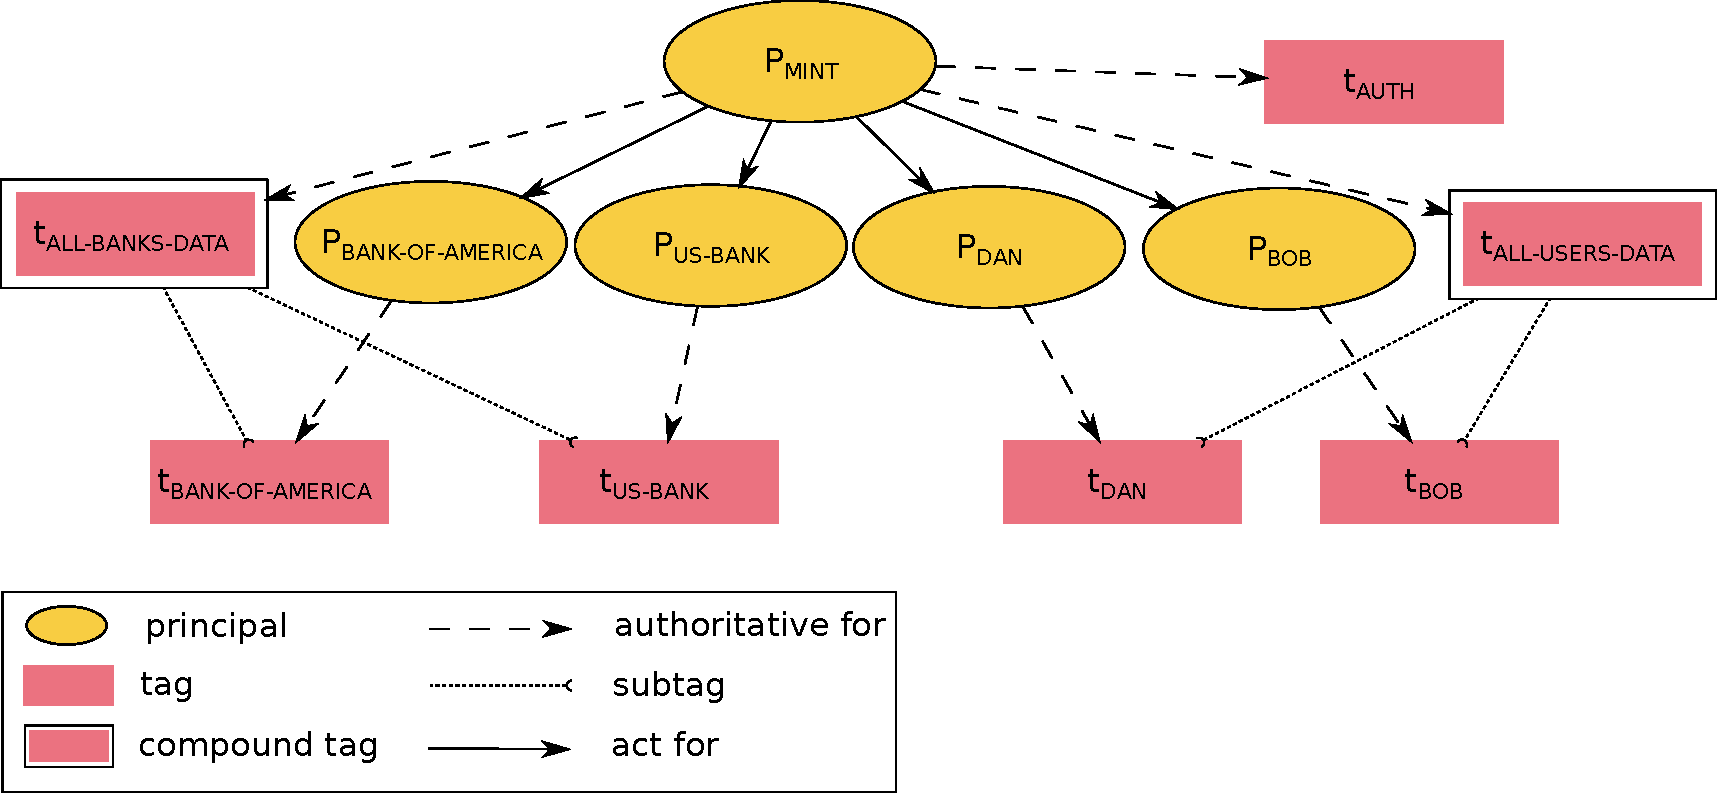
\includegraphics[width=\textwidth,height=\textheight,keepaspectratio]{figures/mint-auth-state-model}
\caption*{Mint Authority State Model}
\caption[Mint Authority State Model]{This diagram illustrates the authority state model of the Mint application in an example where two banks are registered at the application, Bank of America and US Bank. Users Bob and Dan have both signed up. Principals are denoted \emph{P$_{<name>}$} and tags are denoted \emph{t$_{<name>}$}.}
\label{fig:mint-auth-state-model}
\end{figure}


In this section we identify the prinicpals running in the system, the tags associated with different data, and the relationships between them. Figure \ref{fig:mint-auth-state-model} shows an overview of the authority state model for Mint.

An intuitive way to list all necessary\footnote{Neccessary by good design. The application could run with just one principal.} principals, is to think of the different ``clearance levels'' in the system: some information should be accessible by a user, some by a bank, and some information should not be accessible at all. In the light of these requirements, the application employs the following principals:
\begin{description}
  \item[Mint principal] \ \\
    This principal is authoritative for all tags in the system, and is
    used for aggregate analysis of user data and
    user authentication.
  \item[Bank principals] \ \\
    Each of these principals is authoritative for a particular bank's tag.
  \item[User principals] \ \\
    Each of these principals is authoritative for a particular user's tag.
  \item[Public principal] \ \\
    Described in section \ref{aeolus:auth-calls}, this
    principal is used when no privileged operations are 
    necessary to ensure no information leaks.
\end{description}

Similarly, to separate data in the system according to its purpose, (e.g. user password, user bank credentials, etc..), the application employs the following tags:
\begin{description}
  \item[User data tags] \ \\
    Each of these tags is associated with data 
    carrying a particular user's information.
    For example, history of a user's transactions.
    Reading (or modifying) user information
    requires declassifying (or endorsing)
    a user data tag.
  \item[Bank data tags] \ \\
    Each of these tags is associated 
    with data carrying a particular bank's information.
    Reading a user's bank credentials
    requires declassifying a bank data tag. This tag is
    important so that only a bank's closure (a closure
    bound to the bank's principal) is able
    to access a user's bank credentials for authentication.
  \item[All-Users-Data tag] \ \\ 
    This tag is a super tag for all the user 
    tags.
    Running aggregate analysis on Mint user accounts
    requires declassifying this tag.
  \item[All-Banks-Data tag] \ \\ 
    This tag is a super tag for all the bank tags.
    Adding a new bank to Mint requires endorsing
    this tag.
  \item[Authentication tag] \ \\
    This tag is associated with user's Mint passwords.
    Authenticating a user's Mint credentials
    requires declassifying this tag.
    This tag is important to prevent release of
    a user's password to someone who might have
    gained access to their account.
\end{description}

\subsection{Files}\label{sec:mint-fs}

\begin{figure}[h]
\centering
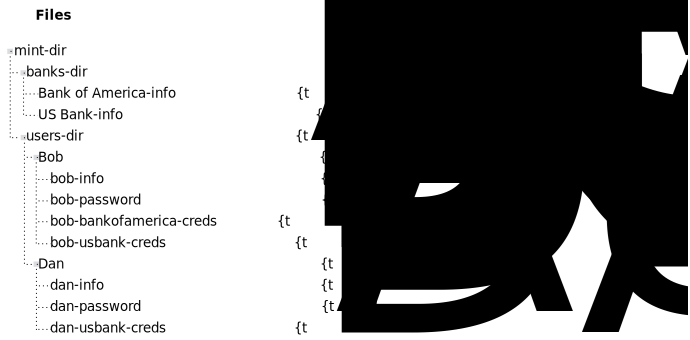
\includegraphics[width=\textwidth,height=\textheight,keepaspectratio]{figures/mint-filesystem}
\caption*{Mint File System Hierarchy}
\caption[Mint File System Hierarchy]{In continuation of the example in figure \ref{fig:mint-auth-state-model}, Bob added credentials for Bank of America and US Bank to his account, and Dan added credentials for US BANK to his account.Tags are shown under the secrecy label and integrity label columns, and are denoted \emph{t$_{<name>}$}. \emph{t$_{BOB}$} and \emph{t$_{DAN}$} are both user data tags. \emph{t$_{BANK-OF-AMERICA}$} and \emph{t$_{US-BANK}$} are both bank data tags. \emph{t$_{AUTH}$} is the authentication tag, and \emph{t$_{ALL-USERS-DATA}$} tag is a supertag as shown in figure \ref{fig:mint-auth-state-model}.}
\label{fig:mint-fs}
\end{figure}

The application uses Aeolus files for persistent storage. Figure \ref{fig:mint-fs} shows the hierarchy of the Mint files and their labels, described below:
%The application stores it's information under a root directory called \emph{mint-dir}.  The are two direct subdirectories of \emph{mint-dir}: \emph{banks-dir} and \emph{users-dir}.

\begin{description}
  \item[\emph{mint-dir}] \ \\
    This is the root directory for the Mint 
    application.
    The secrecy label is empty, the integrity 
    label contains the \emph{ALL-USERS-DATA} and
    the \emph{ALL-BANKS-DATA} tags.
  \begin{description}
    \item[\emph{banks-dir}] \ \\
      Contains a \emph{bank-info} file for each 
      bank that was registered to the 
      application. This 
      directory has an empty secrecy label, and 
      has the \emph{ALL-BANKS-DATA} tag in its 
      integrity labels.
      Each of the \emph{bank-info} files in 
      this directory has a \emph{BANK-DATA} 
      tag in both its secrecy and integrity 
      labels.
    \item[\emph{users-dir}] \ \\
      Has the \emph{ALL-USER-DATA} tag in both 
      its secrecy and integrity labels. Contains 
      a subdirectory per user, each subdirectory 
      contains a \emph{USER-DATA} tag in its 
      secrecy label, and a \emph{USER-DATA} tag 
      in its integrity label.
      Each of these subdirectories contains the 
      following files:
      \begin{description}
        \item[\emph{user-info}] \ \\
          Contains the user tag for that user.
          This file has the \emph{USER-DATA} tag 
          in both its secrecy and integrity labels.
        \item[\emph{user-password}] \ \\
          Contains the user's password.
          This file contains the \emph{AUTH} tag in 
          its secrecy label, and the \emph{USER-DATA} 
          tag in its integrity label.
        \item[\emph{user-bank-creds}] \ \\
          Contains user credentials for a particular 
          bank.
          The \emph{users-dir} directory contains 
          one \emph{user-bank-creds} file per bank 
          the user added to their account.
          This file has the \emph{BANK-DATA} and 
          \emph{USER-DATA} tags in its secrecy label, 
          and the \emph{USER-DATA} tag in its 
          integrity label.
      \end{description}
  \end{description}
\end{description}

\subsection{Shared Memory Objects}
\label{sec:mint-smo}

\begin{figure}[h]
\centering
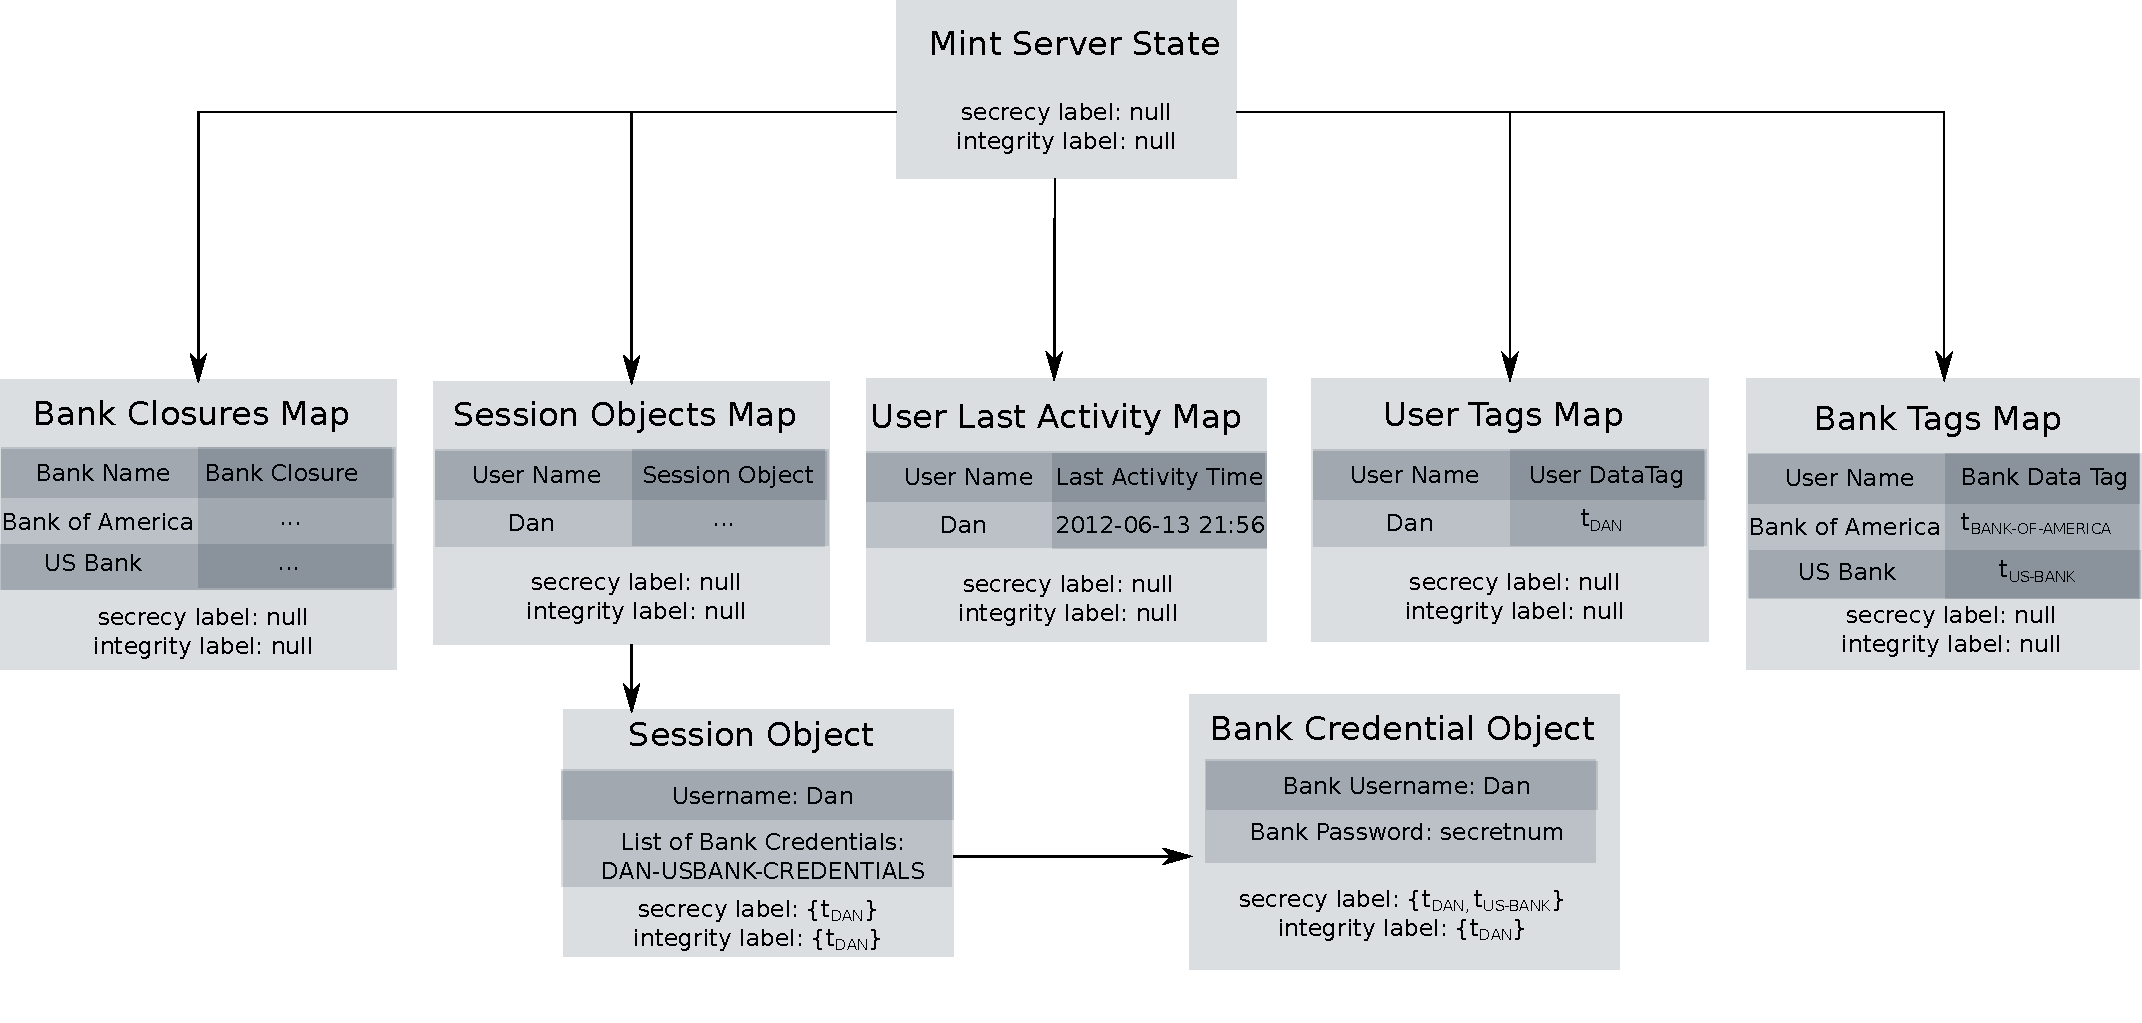
\includegraphics[width=\textwidth,height=\textheight,keepaspectratio]{figures/mint-shared-state}
\caption*{Mint Shared State Objects}
\caption[Mint Shared State Objects]{This figure illustrates what shared memory objects the Mint application uses. This diagram builds on the example presented in Figure \ref{fig:mint-fs}. Bob's session had timed out, and no session object or last activity time is stored for his username. Meanwhile, Dan's session is still active, his session state object is included in shared memory.}
\label{fig:mint-ss}
\end{figure}

To allow for quick responsiveness to user requests, the application stores some key information in shared memory. Figure \ref{fig:mint-ss} diagrams the different shared memory object, their relations and what information they store.

A \emph{Mint Server State} object that has null labels is stored as the Aeolus \emph{root} object and contains the following objects:

\begin{description}
  \item[Bank Closures Map] \ \\
    A bank closure is used to retrieve user
    information from a bank. The bank closure
    is authoritative for the tag of the bank
    it is working for. A bank closure has null
    labels.
    This object maps each bank name 
    to a bank closure, and has null labels itself.
  \item[Session Objects Map] \ \\
    This object maps a username to a session 
    object.
    A \emph{session object} contains session 
    information about a user. It also contains
    a list of \emph{bank credential} objects,
    one for each bank a user has registered 
    for, as well as the user's Principal ID
    (PID). 
    A \emph{session object} has the 
    \emph{USER-DATA} tag in both its labels.
    \begin{description}
      \item[Bank Credentials] \ \\ 
        A \emph{bank credentials} object contains 
        the user's username and password for that
        particular bank. It has a \emph{BANK-DATA}
        tag and a \emph{USER-DATA} tag in its 
        secrecy label, and a \emph{USER-DATA} tag
        in its integrity label.
    \end{description}
  \item[User Tags Map] \ \\
    The application stores the tag for each user 
    that has an active session, this allows the 
    application server to access session objects 
    with the user tag in their label. User tags 
    are stored as a mapping from username to tag.
    This object has null labels.
  \item[Bank Tags Map] \ \\
    Bank tags are important to store in memory to 
    allow for quick server response time. They are 
    stored as a map from bank name to bank tag.
    This object has null labels.
  \item[User Last Activity Map] \ \\
    The time of a user's last activity 
    is used to identify which users
    are still active. This information is stored 
    as a mapping from username to last activity 
    time.
    This object has null labels.
\end{description}

\section{Implementation}
\label{mint:impl}

The application server runs on a VN, and receives user requests via RPC. Users can sign up, login, logout, register a bank and retrieve expenditure statistics.

At startup, the system registers a number of banks. These are the banks which the users can later add accounts for on their Mint account. The system is now ready to accept users.

Users can register to the Mint service through a \emph{signUp} RPC call:

\begin{description}
  \item[\emph{signUp(username, password)}] \ \\
    Signs up a new user with the username as 
    \emph{username} and password as \emph{password}. 
    If \emph{username} is available, associates 
    those credentials with a newly-created user data 
    tag and a newly-created principal ID,
    then stores all this information on disk under
    a new user directory, as per the file system
    hierarchy described in section 
    \ref{sec:mint-fs}. The system
    also stores the newly created tag in the 
    \emph{User Tags Map}.
    Throws an exception if this \emph{username}
    is already used.
\end{description}

Users can then log in to modify their account and retrieve their information using the following RPC call:

\begin{description}
  \item[\emph{login(username, password)}] \ \\
    Authenticates a user, and if successful, 
    stores their information in a session 
    object, and updates their last activity
    time using the shared memory objects
    described in section \ref{sec:mint-smo}.
    The system authenticates the 
    credentials by calling an 
    \emph{authentication closure}, which 
    adds the All User Data tag, 
    verifies the credentials, declassifies 
    and terminates if the \emph{username} and
    \emph{password} are correct, throws 
    an exception otherwise.
\end{description}

Once a user logs in, they only have to include their \emph{username} in pursuing requests to carry out different actions. In each of the following RPC calls, authentication is carried out by checking if the provided \emph{username} has a session that has not timed out yet (there is a last activity time associated with a session, and thus must not be older than a certain amount of time, e.g. 15 minutes).

\begin{description}
  \item[\emph{addBank(username, bankName, bankUsername, bankPassword)}] \ \\
    Registers the specified bank 
    for the specified username with the given 
    credentials.
    This request writes a \emph{user-bank-creds} 
    file to disk, with the tag of
    the user in its integrity label, and the 
    tag of the user and that of the bank
    in its secrecy label.
  \item[\emph{downloadTransactions(username)}] \ \\
    This action connects to each bank the 
    user has registered for their account, 
    downloads the latest transactions for the user, 
    processes them, and returns the result.
    The RPC thread uses the closure of the bank to
    connect to the bank and declassify the 
    information returned. The thread then
    adds a user tag to it's secrecy label, 
    and uses a reduced authority call to 
    the public principal to process the information; 
    this ensures that information
    cannot be leaked while it is being
    processed
    \footnote{One can imagine that the 
    information is being processed by a different
    application in the system, 
    using this technique means our application 
    does not have to trust that 
    application.}. 
%    Figure x shows a code sample.

%  \item[\emph{attack(attacker, victim)}] \ \\
%    \emph{Attacks} the uer specified by \emph{victim}. 
%    This request aims to simulate a bug 
%    in the appliction that mistakingly 
%    delegates the victim's 
%    data tag to the attacker's principal.
%    This user action is useful for testing 
%    and auditing purposes, as explained later
%    in this chapter.

  \item[\emph{logout(username)}] \ \\
    Terminates the user's session, removing 
    their information from shared memory.
  \item[\emph{removeBank(username, bankName)}] \ \\
    Removes the specified bank from a user's account.

\end{description}

\noindent
For each RPC call, the thread handling the call starts running on behalf of \emph{P$_{MINT}$}, and then reduces its authority as soon as possible to avoid errors leading to information leakage. For example, in \emph{downloadTracations}, after authenticating the user, the thread reduces its authority to run on behalf of the users principal, then processes the downloaded information on behalf of \emph{P$_{PUBLIC}$} and then returns.


\section{System Security}

The use of a \emph{username} in the implementation of the RPC calls defined above to identify which user invoked those calls creates a vulnerability in our system. Alice could send a \emph{downloadTransactions(``Bob'')} request, and because the information is being sent outside the Aeolus system, the information in the reply would have null labels, and hence Alice could access Bob's information.

Another problem that comes up is related due to the assumption that the user is connecting from another Aeolus node. If this was not the case, i.e. the requests are coming from outside the Aeolus system, sensitive information would be exposed over the network (e.g. the user's Mint credentials), which wouldn't happen for RPCs within the Aeolus system because those are encrypted\footnote{Requests coming from outside the system could be RPC or HTTP requests.}.

Both issues can be resolved by using standard cryptography mechanisms to encrypt and authenticate external communication. For example, encrypting all requests and replies coming in and out of the system and, in addition, sessions can be identified by unguessable temporary session-ids, and, those session-ids would be used to authenticate future requests in that session.

Finally, the security of application can be improved by introducing more principals to the authority state model to make the information flow control more fine-grained. For example, we could separate the authority to register banks from the authority to authenticate users.

\appendix
%\chapter{Tables}

\begin{table}
\caption{Armadillos}
\label{arm:table}
\begin{center}
\begin{tabular}{||l|l||}\hline
Armadillos & are \\\hline
our	   & friends \\\hline
\end{tabular}
\end{center}
\end{table}

\clearpage
\newpage

%\chapter{Figures}

\vspace*{-3in}

\begin{figure}
\vspace{2.4in}
\caption{Armadillo slaying lawyer.}
\label{arm:fig1}
\end{figure}
\clearpage
\newpage

\begin{figure}
\vspace{2.4in}
\caption{Armadillo eradicating national debt.}
\label{arm:fig2}
\end{figure}
\clearpage
\newpage

%% This defines the bibliography file (main.bib) and the bibliography style.
%% If you want to create a bibliography file by hand, change the contents of
%% this file to a `thebibliography' environment.  For more information 
%% see section 4.3 of the LaTeX manual.
\begin{singlespace}
\bibliography{main}
\bibliographystyle{plain}
\end{singlespace}

\end{document}

